\chapter{Platform Design}
Obtaining successful flight results with an aerial vehicle will need both precise control algorithms and a robust platform. This chapter contains the technical details of how the final platform decisions was made. The final design will be compared and validated against the proposed outcomes stated above. 

\section{Factors Affecting Design Decisions}
\todo[inline]{not sure about the name of this section}
Before a proper analysis can be done, certain criteria need to be outlined. These include aspects of the project such as the required flight time and manoeuvring decisions. These factors have been drawn up from the proposed research questions and end use case.

\subsection{Physical Restrictions and Requirements}
One of the major components \projectName will have to overcome is to navigate these unknown areas and not only survive collisions, but also reject the disturbances introduced by being close to the walls. Since mine shafts are predominantly long and narrow, the same approach will be looked at for the design of the drone. Hence the platform will be made to be long and narrow. The unique disturbances found in a mine also help define the end configuration as it needs to be able to withstand these disturbances.
Since the drone will be required to navigate very confined spaces, the smaller the drone the better. The minimum size of the drone is limited by the need for adequate flight time as well as payload capacities.

\subsection{Manoeuvring Decisions}
The manoeuvring decisions are dependant on the type of environment and type of missions required by the platform. These decisions influence the final design of the craft.
The end use case for \projectName will include mapping of unknown areas. To complete this, it will simplify the procedure if the drone keeps it's orientation during flight. Due to the nature of the environment, fast speeds will not be used regularly. Therefore \projectName will be designed to have slow, steady and controlled movements. More is discuss in the flight strategy section.

\subsection{Disturbances}
As described above the discussions with CSIR lead to the decision to attempt to use this drone in a mine. Apart from the difficulty of navigating and manoeuvring through an unmapped area there are other disturbances introduced into the system. 
Due to the nature of the tunnels, wind gusts are created that funnel through these passageways. They can reach speeds of up to \todo{Insert Gusts Speed and reference}. Due to the direct relationship between thrust and initial velocity as shown in \eqref{EQ_ThrustMass} any change in wind speed through the rotors will unbalance them.
The effect of coming close to a wall of floor has been discussed in the literature study. The near wall effect will also create an imbalance that creates a moment towards the wall. 
Since the areas will be unknown, collisions and bumps are extremely likely, if not inevitable. The drone must be able to withstand a collision and maintain it's orientation as best as possible.

\subsection{Thrust Overhead}
The total overhead of a rotorcraft is a percentage above the thrust required for hover. This value determines a craft's ability to manoeuvre, with a higher value giving it more freedom and a greater ability to resist disturbances. With these benefits the system does become very sensitive and more difficult to control and stabilise. Since the craft will be in confined narrow passages, the craft does not need to be fast moving. Rather a "slow and steady" pace will be approached. The craft does however need enough power to counteract the disturbances described above. These considerations lead to a value of $150\%$, with $100\%$ being enough thrust to hover. \todo[inline]{Back this up with references from other designs, spoken about later consider removing from here. Maybe reference botom section?}

\subsection{Flight Time}
Flight time is dependant on efficiency/power requirements of the system as well as the capacity of the on-board power source. This is where the designer runs into a catch 22. By adding a larger power source the weight is increased and therefore the platform requires more power to keep itself aloft. Weight is a determining factor for any aerial system and influences flight time, for this reason the weight of every subsystem must be optimised. To ensure the craft can complete a mission it will need a decent flight time. Initial conversations have set 30 minutes as the bottom limit. The original platform might not be able to reach this goal, but once the platform is performing adequately adjustments can be made to the system to optimise weight and power consumption. 

\section{Final Concept Choice}
The traditional configurations of drones are incapable of handling disturbances introduced by being in a confined space and will continue to struggled to overcome this problem\todo{Maybe a bit harsh, but need to validate why we're not using a standard design}. For this reason a few unique designs were considered and a lot subsequently rejected. Although some rejected ideas did help define the final configuration.

\subsection{Rejected Designs}
\subsubsection{Gimball}
The Gimball design as shown in Figure \ref{IM_Gimball} has been discussed thoroughly in the literature. It is definitely the most sophisticated close quarter drone in the world today. It's rolling cage and gimbal design reduces collisions to hardly effect the drone's flight paths at all. Unfortunately it's Co-axial rotors limit the payload capabilities and reduce efficiency of the craft which inhibits the total flight time. The rolling cage also prohibits successful mapping as the orientation of the craft is constantly changing and any sensors inside the cage will be obscured by the rolling protection.

\begin{figure}[H]
\centering
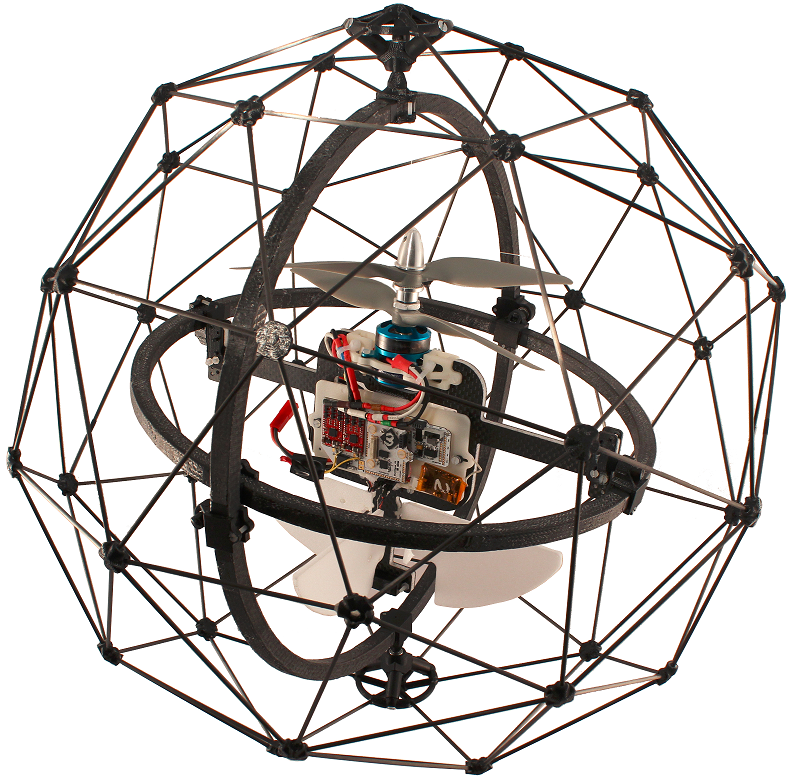
\includegraphics[height = 6cm]{Images/Design/Gimball}
\caption{Flyability's Gimball (Picture taken from http://www.flyability.com/product/)}
\label{IM_Gimball}
\end{figure}

The Gimball is a great tool and will aid a lot of industries, but it was not seen as a viable method to conduct mapping or carry any sort of payload for an extended period of time.

\subsubsection{Tandem Tilt Rotors}
After much thought into the problem a unique design was considered. Figure \ref{IM_TiltTandem} is the initial realisation of that concept. The idea was to capitalize on a tandem's narrow design while giving it more freedom by allowing the rotors to tilt. After the concept had been drawn up it was noted that adding tilt abilities to standard configuration has been looked at and used successfully before \cite{TandemTiltRotor, TripleTiltRotor}.

\begin{figure}[H]
\centering
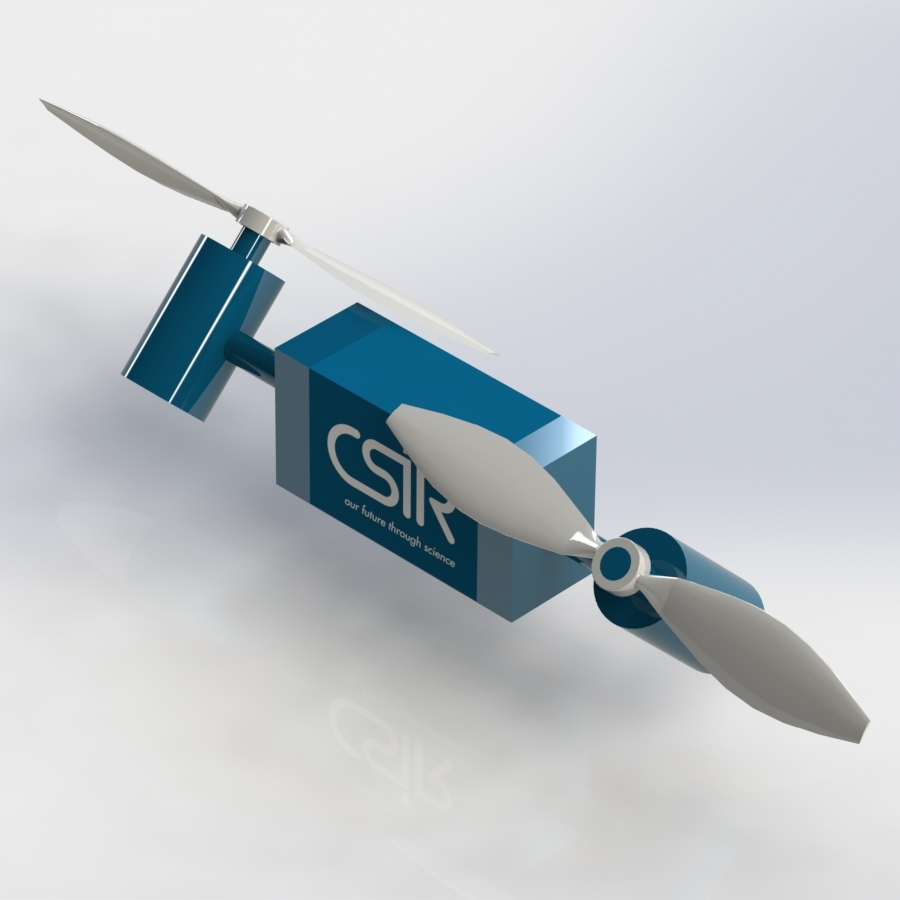
\includegraphics[height = 6cm]{Images/Design/Tandem}
\caption{Rendering of initial concept of the Tandem Tilt rotor Rotorcraft}
\label{IM_TiltTandem}
\end{figure}

The big issue with this design would be controlling the platform. Designing a tilt rotor without variable tilt rotors would not produce enough roll control. The tilt mechanism will help with this, but affect too many other efficiencies while doing it. The tandem will also be more susceptible to disturbances than a four rotor approach.

\subsection{Chosen Concepts}
\todo[inline]{For the comparison, figures were obtained while the following was assumed: Thrust to RPM linear. RPM to current linear. Make sure they are correct}

After much thought two concepts were selected as final candidates. This next section walks through some of the important factors considered and ultimately, why certain decisions were made. 
On the left of Figure \ref{IM_UnlikeSizes} represents the \textit{"Unlike Size Quad"} and the right of Figure \ref{IM_UnlikeSizes} is the \textit{"Overlapping Quad"}. 

\begin{figure}[H]
\centering
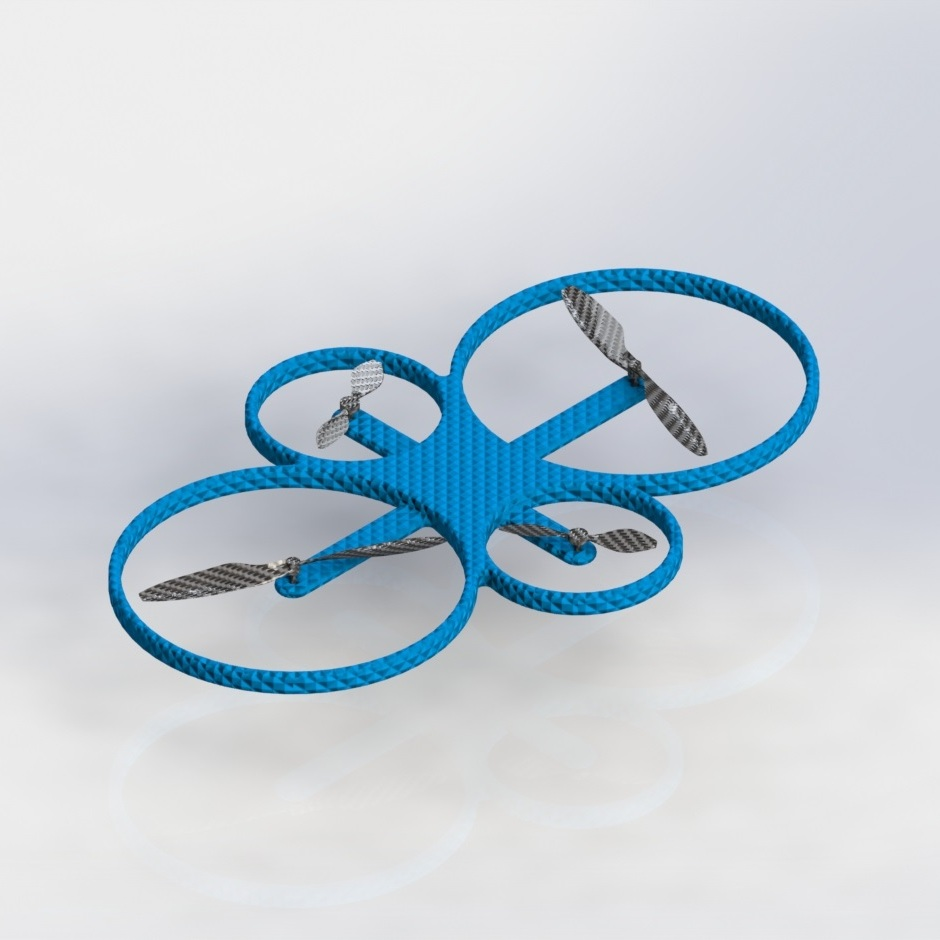
\includegraphics[height = 6cm]{Images/Design/UnlikeSizes}
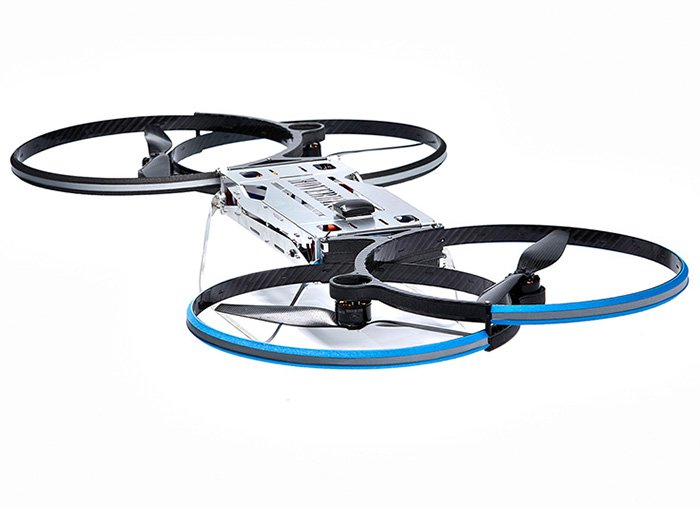
\includegraphics[height = 6cm]{Images/Design/Overlapping}
\caption{a)Rendering of initial concept of the unlike rotor size quadcopter and b) Malloy Aeronautics Hoverbike Concept (Picture taken \cite{MAHover}).}
\label{IM_UnlikeSizes}
\end{figure}


\subsubsection{Concept 1 - The Overlapping Quad}
The overlapping quad is a concept pursued by Malloy Aeronautics \cite{MAHover}. They used the design in an initial concept of their hover bike. The design uses an X-formation for it's rotors, except the rotors are brought in to limit the width of the craft to the point that they overlap, as shown in Figure \ref{IM_UnlikeSizes}. Each overlapping pair will have both spin directions, this feature is shown in Figure \ref{IM_OverlappingPair}.

\begin{figure}[H]
\centering
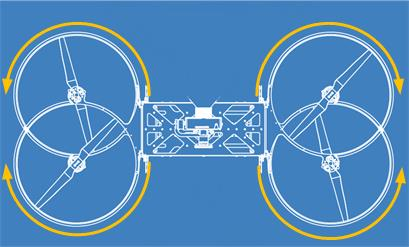
\includegraphics[height = 6cm]{Images/Design/OverlappingVD}
\caption{Overlapping concept, visual representation of rotor pairs. Image modified from \cite{MAHover}}
\label{IM_OverlappingPair}
\end{figure}

If this configuration is selected, there are still other design questions that need to be answered. Overlapping rotors introduce an inefficiency into the system. Johnson in \cite{HeliTheory}, says there is much debate in how the efficiency is calculated. He states two of his preferred methods, the method chosen has a better approximation for small overlaps and is shown in \eqref{EQ_OverlapEfficiency} \cite{HeliTheory}. $\Delta P$ is the interference power (considered here as a fraction of total power) and $m$ is the overlap fraction and is calculated in \eqref{EQ_Overlap} \cite{HeliTheory}.

\begin{equation}
\label{EQ_OverlapEfficiency}
\frac{\Delta P}{P} = (\frac{2}{2-m})^{1/2} - 1
\end{equation}

\begin{equation}
\label{EQ_Overlap}
m = \frac{2}{\pi} \Bigg[ \cos^{-1}\frac{l}{2R} - \dfrac{l}{2R}\sqrt{1 - {\dfrac{l}{2R}}^2} \Bigg]
\end{equation}

These quantities assume a small vertical separation so that the inflow rates of both rotors can be considered the same. To calculate the overlap function, the rotor radius $R$ is needed as well as the separation distance $l$. Figure \ref{IM_SeperationGraph}, illustrates how the separation affects both the  overlap function as well as the total power as a percentage.


\begin{figure}[]
\centering
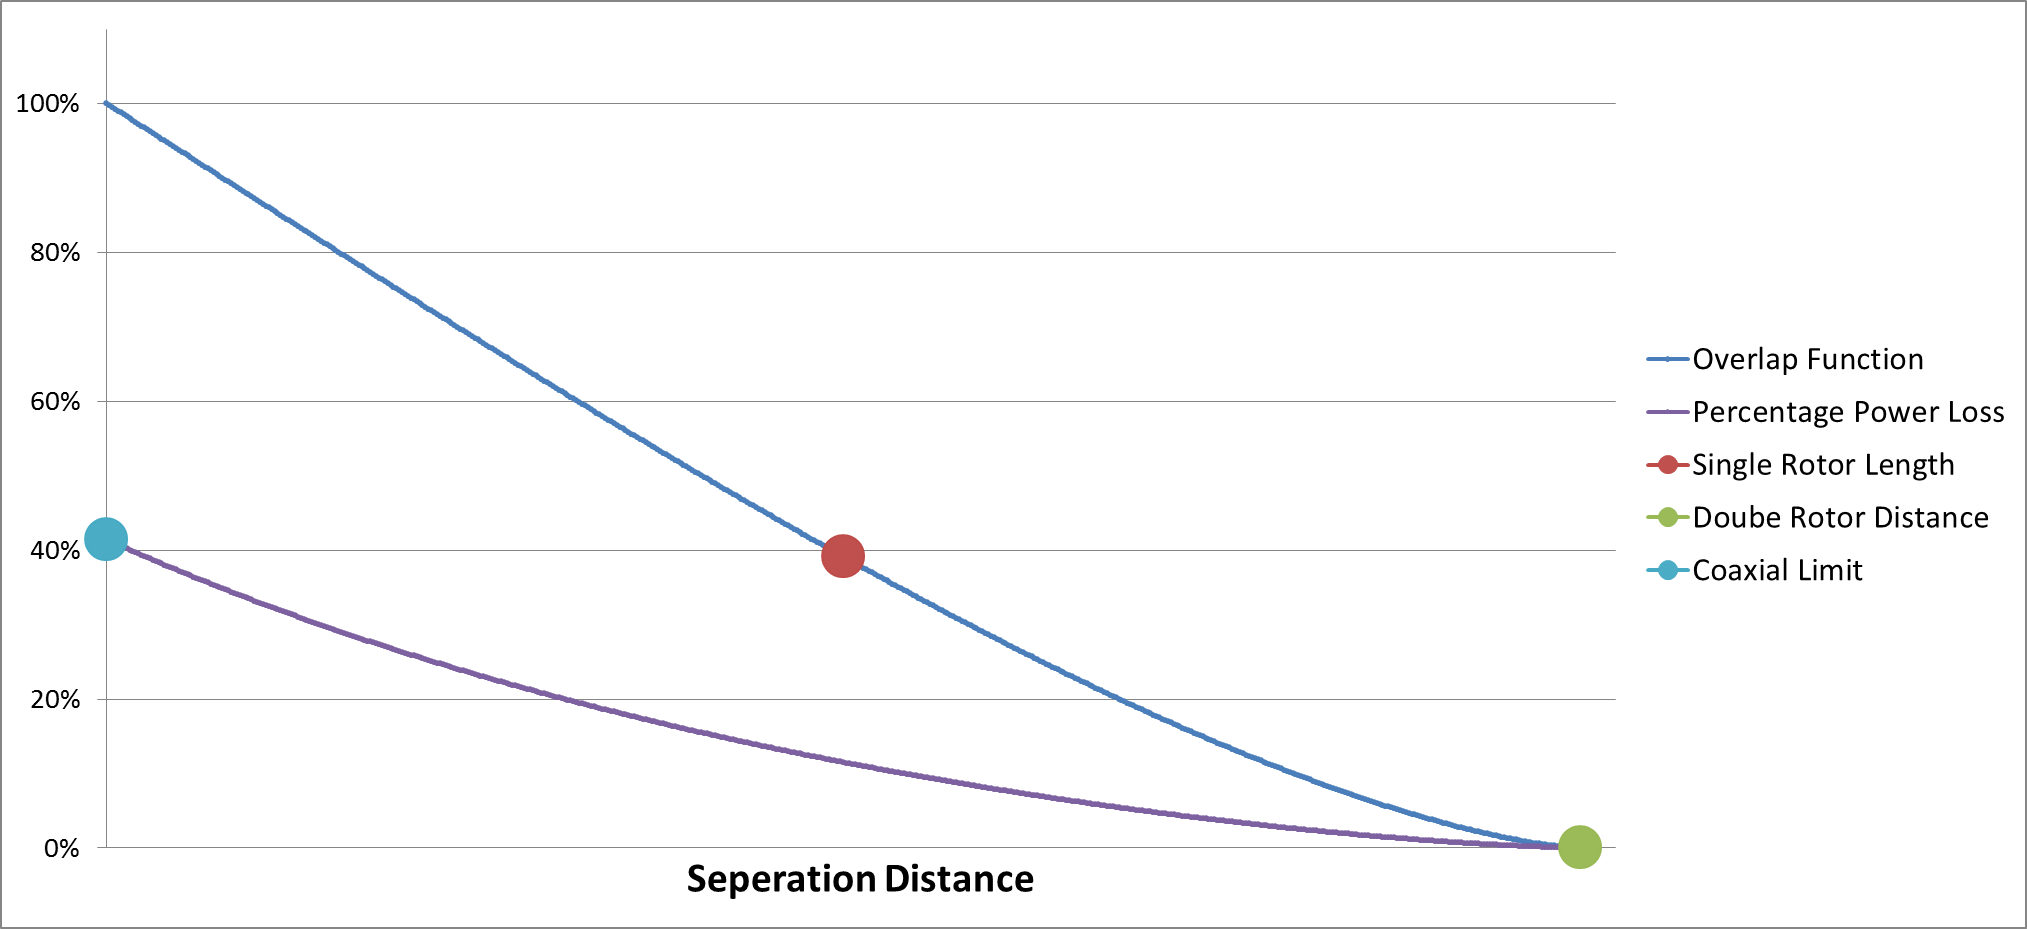
\includegraphics[height = 6cm]{Images/Design/SeperationGraph}
\caption{Graph representing the effects of separation distance in an overlapping quad}
\label{IM_SeperationGraph}
\end{figure}


The length of the craft needs to also be decided, this aspect only becomes critical once payload requirements are factored in. As stated above, this design was an initial concept for a hoverbike with the intended payload capacity of a human. So a big positive to this design is the power to size ratio. This benefit can be utilised through handling larger payloads, or a larger battery pack increasing total flight time.

\subsubsection{Concept 2 - The Unlike Size Quad}
The unlike size quad is an original design that uses the standard cross formation, except it has two pairs of different size rotors. This means that the counter rotating pairs will be set up as shown in Figure \ref{IM_UnlikeSizePair}, with each rotation direction having one big and one small rotor. 

To maintain a common DL in the system the thrust requirement will be lower on the smaller blades and larger on the bigger blade. The smaller the side rotors get, the higher the thrust requirements of the larger rotors become, this limits the rotor size ratio. Initial calculations, factoring in thrust overhead, overall size of the craft and minimum thrust allowed to rotors, set the ratio between $65\% - 80\%$.  When approaching the lower bound, the thrust requirement for hover alone leaves very little room for manoeuvring or disturbance rejection. The upper bound reaches a point where the size difference is so negligible the design's narrow intent is lost.

\begin{figure}[H]
\centering
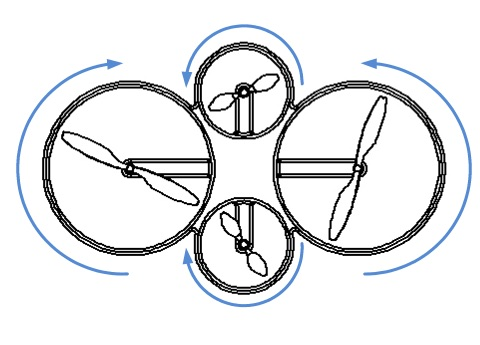
\includegraphics[height = 6cm]{Images/Design/UnlikeSizeRotorPair}
\caption{Unlike Size Quad visual representation of rotor pairs}
\label{IM_UnlikeSizePair}
\end{figure}

The second important choice is how far to put the rotors away from the centre. As the craft gains translational speed, the air doesn't come in directly from the top any more as shown in \ref{IM_MomentumTheoryAirFlow}. Instead it now starts to come in at an angle. As the craft then manoeuvres and changes it's orientation, the air starts coming in at more extreme angles. If the electronics housing has a lot of height it can interfere with the wake boundary and create an inefficiency. This inefficiency is also based on how far the rotors are from the housing. A similar concept is described in Section \ref{SSSECT_NearGroundEffect} Therefore, before this decision can be made the limits of how small the centre electronics housing needs to be decided. 

Through discussions and observations of current systems a minimum limit of $75mm \times 75mm$ was set. To avoid overlap, the distance from the centre of the big rotor and the centre of the craft will be at the very least $R$. Including space for the housing increases this.

The left and right placement is where the originality comes in. Since the craft needs to remain narrow, the side rotors can be brought in as well as shrunk. This would require pushing the two larger rotors slightly more out. Bringing the side rotors in closer to the middle housing will reduce efficiency, so a compromise must be chosen between width and efficiency. Since the side rotors don't contribute as much to the system as their bigger counterparts they have the option of a lower separation distance. The lower separation distance can also be justified by the lower need and use of roll moments and side translations.

Lastly the rotor pitch angle needs to be selected. The major contributing factor of any rotor (besides it's size) is it's pitching angle. As the pitch angle changes, so does the lift to drag ratio. Generally a craft would always want a higher lift to drag ratio, in this case however the side rotors might have a lower lift to drag ratio so they can help counter the torque applied by the larger blades more effectively.

\subsection{Concept Comparison}
After being introduced to the two concepts, they will now be compared based on certain factors. This comparison includes hover efficiency, thrust and electrical power. Lastly size and manoeuvrability are grouped together since they inherently affect each other. The final decision will need to be made with certain assumptions in mind, that must be validated through testing further down the line. These assumptions as well as the method of comparison are described below. 

\subsubsection{Assumptions and Method}
Since both designs use 4 rotors they can be compared relative to a well known design, the standard quadrotor. For each configuration certain parameters need to be decided before a comparison can be done. Using formulas and plots in Microsoft Excel\texttrademark, both designs could be visualised rudimentary as shown in Figure \ref{IM_Excel}.

\begin{figure}[H]
\centering
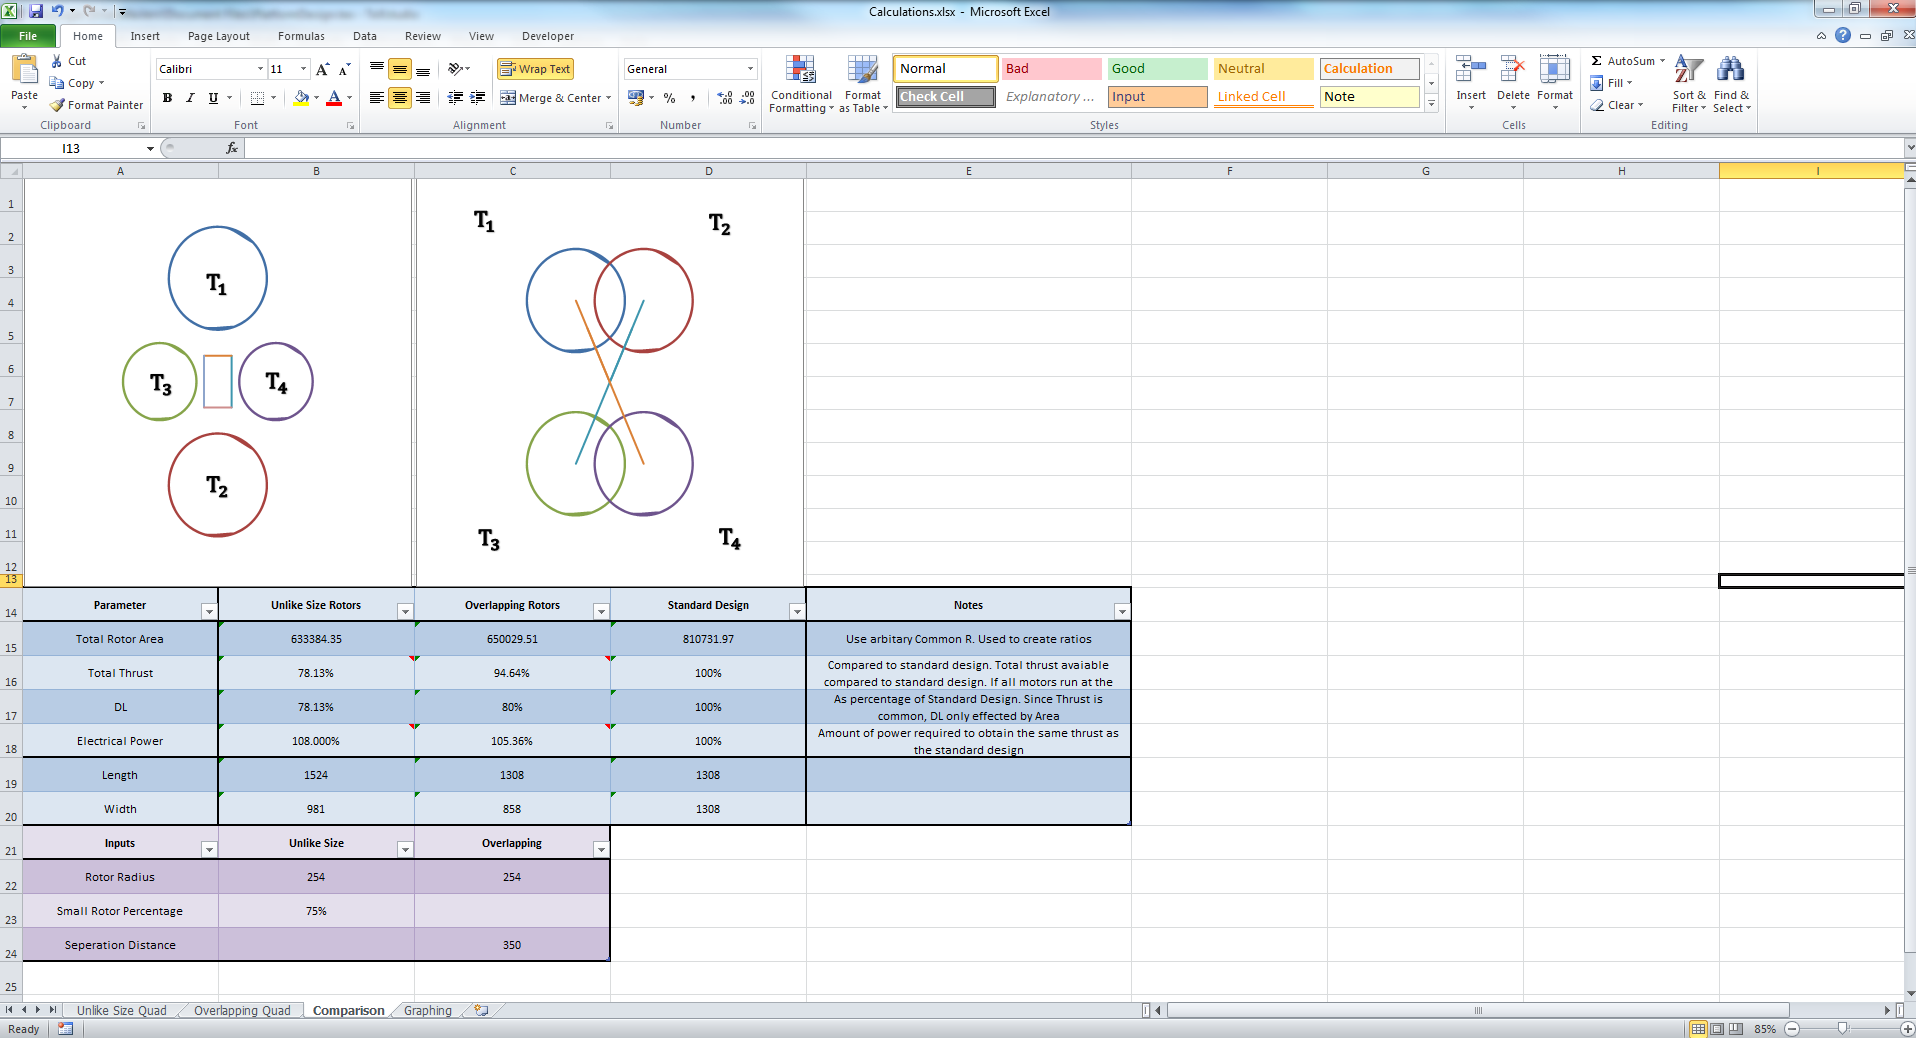
\includegraphics[width = 15cm]{Images/Design/Excel}
\caption{Rudimentary Visualisation of the two concepts using Microsoft Excel\texttrademark}
\label{IM_Excel}
\end{figure}

If hover is a thrust of $100\%$, the overhead was set at $50\%$ \todo{Try and find papers stating other values I want to validate this decision} of that, to a total of $150\%$. Minimum thrust per rotor was set at $20\%$. The mass in question includes provision for a sensor pack of undecided mass. 

The two designs had different decisions that needed to be made. After a bit of trial and error the unlike size quad had it's small rotors set at $75\%$ of the larger ones, this decision is explained further in the text. Just to give a quantifiable reference, R was set at $254mm$. With that assumption the unlike size quad moves it's side rotors in to a distance of $300mm$ and the larger rotors were moved to $508mm = 2R$ away. The overlapping quad set a separation distance of $350mm$ which created an overlap factor of $m = 19.82\%$. 

These values were used to do the following analysis.


\subsubsection{Rotor Area and Disk Loading}
If a rotor size of $R$ is assumed for the rotors\footnote{The big rotors in the case of the unlike size quad} then the total area for a standard quad will be $A_{std} = 4 \pi R^2$. Based on simple geometry, the reduction in radius of the two smaller rotors leads of the unlike size quad leads to a decrease in area. Using $75\%$ this is calculated to $78.13\% of A$. 

As described in \eqref{EQ_Overlap}, the overlapping quad introduces a reduction in total disk area, with an overlap factor of $19.82\%$ leaves a total area of $80.18\%$. Since the thrust requirements are assumed the same, the disk loading ratios will be exactly the same as the area ratios.

\subsubsection{Thrust and Power Considerations}
The $75\%$ decision was based on observation of thrust ratios and comparing them to the minimum and maximum values stipulated earlier. This decision must also be influenced by available rotor sizes and pairings. The final value graphs are shown in Figure \ref{IM_ExcelGraphs}. The thrust percentage per rotor is shown, the points marked are at minimum, hover and maximum. Equation \eqref{EQ_ThrustMass} states that thrust is proportional to area. Therefore the reduction in rotor area will cause a directly related reduction in thrust. The total thrust available to the unlike size quad is $\approx 78\%$ of the thrust available to the standard design. This reduced value also comes at a weight reduction. The overlapping quad has an equal total rotor area but an inefficiency is introduced by the overlap as according to \eqref{EQ_OverlapEfficiency}. Therefore the overlapping quad has $94.64\%$ of the total thrust, without the weight reduction.

\begin{figure}[H]
\centering
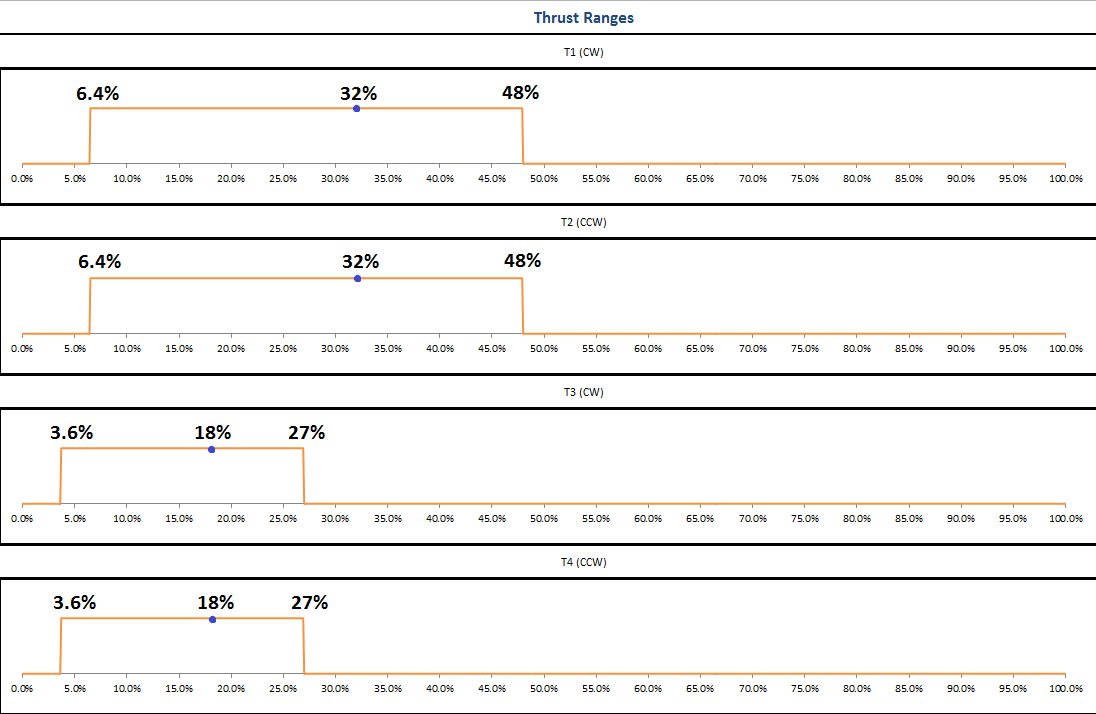
\includegraphics[height = 10cm]{Images/Design/ExcelGraphs}
\caption{Graphical representations of the thrust ratios for the unlike size quad}
\label{IM_ExcelGraphs}
\end{figure}

As for the electrical power, the values were calculated according to how much energy would be needed to obtain the same thrust as the standard design. The inefficiency introduced by the overlap relates to a reduction in thrust of $\Delta T_{overlap} = 5.36\%$, therefore $\Delta P_{overlap} = 14.21\%$ is needed to overcome this loss, based on \eqref{EQ_ElectricalPowerThrust}. 

For the unlike size quad, the reduction in rotor size leads to a substantial loss in aerodynamic power, even with a small reduction in inertia. To regain that power, the rotors need to be pushed harder, this leads to an increase in electrical power. A value of $\Delta P_{unlike size} = 18.5\%$ can be calculated under certain assumptions.

\subsubsection{Size and Manoeuvrability}
The size was calculated as though the drone made a rectangular box and with the rough values above, Table \ref{TAB_SizeComparison} puts those values in a tabular format.

\begin{table}[H]
	\centering
	\begin{tabular}{l | c | c }
		Concept & Length ($mm$) & Breadth ($mm$) \\
		\hline\hline
		Unlike Size	   	& 1524 & 981 \\
		Overlapping    & \boldmath$1308$ & \boldmath$858$ \\
		Standard		& 1524 & 1524\\
	\end{tabular}
	\label{TAB_SizeComparison}
	\caption{Table representing the size comparison of the two concepts}
\end{table}

As shown Both crafts are similar in size, with the overlapping design being slightly shorter as well as more narrow. 

This narrowness comes at a cost. Moments ($M$) are created by a difference in forces($\Delta$) and is multiplied by the distance between the forces ($l$) $M = \Delta Fl $. In the case of the overlapping rotors, the distance between the two different thrust vectors is not as tangible as the unlike size design. This gives the unlike size quad the advantage as bigger moments can be created\todo{Need to make this quantifiable}, allowing for more advanced manoeuvrability and disturbance rejection. However in the case of the near wall effect, the disturbance is created by effecting only one rotor . In the case of the overlapping rotors, the disturbance might be slightly diminished as both rotors will feel the effect. This can be verified later by comparing gathered data to literature. \todo{Would be cool to come back and do this later and reference it here}


\section{Platform Conclusions}

The quantifiable values are culminated below in Table \ref{TAB_ConceptComparison}. The winner of each parameter is written in bold.

\begin{table}[H]
	\centering
	\begin{tabular}{l | c | c | c | c | c }
		Concept & Disk Loading & Total Thrust & Electrical Power & Length ($mm$)& Width ($mm$) \\
		\hline\hline
		Unlike Size	  & \boldmath$78.13\%$  & $78.13\%$ 	& $118.57\%$	& $1524$ & $981$ \\
		Overlapping    & $80.18\%$ & \boldmath$94.64\%$  & \boldmath$114.21\%$	& \boldmath$1308$ & \boldmath$858$ \\
		\hline\hline
		Standard		& $100\%$ 	& $100\%$  	  & $100\%$			& $1524$ & $1524$\\
	\end{tabular}
	\label{TAB_ConceptComparison}
	\caption{Table representing the end comparison of the two concepts}
\end{table}

Now to make the final decision all the factors need to be included. What is known now is that the overlapping quadrotor is superior in almost every quantifiable way. The manoeuvrability aspect is not critical to this application as the use case will involve extremely steady flight. The disturbance rejection of both crafts will be good with 4 rotors. 

Malloy Aeronautics sell what is called a \textit{Drone-3 Kit}, it includes various accessories to help developers use the platform. The novelty of the unlike size rotor quad can now be seen as a negative since it requires a custom frame and shroud.

Based on the above analysis and conclusions the overlapping quadrotor design will be used as the design going forward.

\section{Drone 3}
\subsection{Assembly}



